\documentclass{sigchi}


% Arabic page numbers for submission.
% Remove this line to eliminate page numbers for the camera ready copy
%\pagenumbering{arabic}


% Load basic packages
\usepackage{balance}  % to better equalize the last page
\usepackage{graphics} % for EPS, load graphicx instead
\usepackage{times}    % comment if you want LaTeX's default font
\usepackage{url}      % llt: nicely formatted URLs

% llt: Define a global style for URLs, rather that the default one
\makeatletter
\def\url@leostyle{%
  \@ifundefined{selectfont}{\def\UrlFont{\sf}}{\def\UrlFont{\small\bf\ttfamily}}}
\makeatother
\urlstyle{leo}


% To make various LaTeX processors do the right thing with page size.
\def\pprw{8.5in}
\def\pprh{11in}
\special{papersize=\pprw,\pprh}
\setlength{\paperwidth}{\pprw}
\setlength{\paperheight}{\pprh}
\setlength{\pdfpagewidth}{\pprw}
\setlength{\pdfpageheight}{\pprh}

% Make sure hyperref comes last of your loaded packages,
% to give it a fighting chance of not being over-written,
% since its job is to redefine many LaTeX commands.
\usepackage[pdftex]{hyperref}
\hypersetup{
    pdftitle={SIGCHI Conference Proceedings Format},
    pdfauthor={LaTeX},
    pdfkeywords={SIGCHI, proceedings, archival format},
    bookmarksnumbered,
    pdfstartview={FitH},
    colorlinks,
    citecolor=black,
    filecolor=black,
    linkcolor=black,
    urlcolor=black,
    breaklinks=true,
}

% create a shortcut to typeset table headings
\newcommand\tabhead[1]{\small\textbf{#1}}


% End of preamble. Here it comes the document.
\begin{document}

\title{Visual Design for Economic Labor Measurement Report}

\numberofauthors{3}
\author{
  \alignauthor Benjamin Bengfort\\
    \affaddr{University of Maryland}\\
    \email{benjamin@bengfort.com}
  \alignauthor Xintong Han\\
    \affaddr{University of Maryland}\\
    \email{hixintonghan@gmail.com}
  \alignauthor Assaf Magen\\
    \affaddr{University of Maryland}\\
    \email{amagen@umd.edu}
  \alignauthor Hao Zhou\\
    \affaddr{University of Maryland}\\
    \email{zhhoper@gmail.com}
}

\maketitle

\begin{abstract}
Visualizing employment statistics (e.g., unemployment rate, labor force) is of great importance, since it can be used to help people gain a better understanding of  the economic situation and measure the economic and political solutions. In this project, we design a web application to visualize the employment situation of the United States. This application provides a heat map of the United States to show the employment situation of different states, as well as a dashboard with line charts to show them as time series. Furthermore, another view called wealth of nations plays a complementary roll of the heat map to show the employment situation for different states in US. The web application is primarily written in JavaScript using D3 with a small Python web server sending JSON data to the D3 front-end. It also has a data ingestion component, allowing quick data gathering from the BLS and from the monthly job release. Moreover, two rounds usability studies with 8 volunteers are conducted to help the project development. It is our hope that our project will eventually be hosted by some organization like Urban Institute and used widely by journalists and researchers.
\end{abstract}

\keywords{
	Employment Situation; Information Visualization; D3
}


\section{Introduction}
The Employment Situation Report is a critical, monthly assessment of the state of labor in the United States. In recent years, this report has been used to measure economic and political solutions to the 2008 downturn, as well as the performance of politicians themselves. News media hypes the publication of the report each month, and then follows the publication with widespread analyses and critiques.

However, this report, based on two surveys of the Bureau of Labor Statistics (BLS), does not allow meaningful exploration or insights as it is published in PDF form, which consists of mostly tables. In this project, we utilize the data provided in these surveys to create an ``employment dashboard'' which called ELMR (Economic Labor Measurement Report) that allows interactive analysis of the current employment situation of the United States, as well as providing historical context by utilizing previous month employment reports (and a slider allowing you to navigate in time). This dashboard consists of four parts: Time Series, Geography, Wealth of Nations, and Export Data. The Time Series view, users can choose two different statistics to visualize and compare them over time. In the Geography view, a map of the United States is used to specifically visualize how the employment changes regionally, and allows users to gain insights into the employment situation for different states and regions. In addition to that, the Wealth of Nations part shows the employement level, size of labor force and unemployment rate in a bubble chart, . Finally, users can use the Export Data part to download the data sets they want to explore in csv form. One important feature of this web application is that we can update the monthly released data by BLS, so users can visualize and explore the up-to-date employment situation.


\section{Related Work}

\subsection{Employment Situation Visualization}
Visualizing the employment statistics, such as employment rate, job gains, etc. is of great importance, it can give people especially government officials a better understanding of the employment situation and economic environment. As a result, plenty of works have been done to address this problem. On its website \cite{Labor_data}, Bureau of Labor Statistics (BLS) provides tables and line charts that enable users to see how one specific data changes overtime. In addition, it also provides a monthly report that gives people a glance of the up-to-date data and changes. However, it is very hard for users to find insights only with one line chart along with a table, because they cannot compare different statistics at the same time and interact with the data. Also, the report which is a PDF form does not allow informative insights and explorations. If users want to visualize these data, they have to download them and make use of some other visualization tools to find the information they want. Also, sometimes even finding the dataset of interest is difficult since users have to go back and forth in the website and very easy to get lost.

To this end, Urban Institute \cite{urban_website}, as well as some visualization galleries like \cite{David2014, Jeremy2014,Tableau}, use the public published employment data to generate interactive visualizations. For example, \cite{Jeremy2014} uses 255 charts to help people explore how recession reshaped the economy, where each line in the visualization shows how the number of jobs has changed for a particular industry over the past 10 years. In this way, users can find how the recession reshaped the nation’s job market industry by industry. These works are very powerful in visualizing employment statistics to people. Nevertheless, using these existing approaches, users cannot choose the data dimensions of their own interest and find insights by leveraging different visualization techniques. Moreover, most of these methods are not easily updatable when BLS releases new data every month. To address these problems, in this project we create a web application to help users explore the employment situation by choosing and explore the data of their own interest, and the data can be automatically updated when BLS release its monthly new data.


\subsection{Time Series Data Visualization}
Since the employment statistics are mostly time series data, some papers \cite{Few2007,Roger2008,Jeremy2014} about visualizing time series are also related to our project. \cite{Few2007}  gives us a brief idea of which patterns of change we should pay attention to for time series data; \cite{Roger2008} shows how to visualize multi-dimensional time series data with different location information; and \cite{Jeremy2014} focuses on visualizing the job change during the recession, which is very similar to part of what we want to visualize.


\subsection{Geolocation-Based Data Visualization}
For many users, they may want to visualize and compare the data for different regions or states. For example, a user may want to see how the unemployment ratio changes in the state where he or she lives. As a result, an informative visualization should give the option that users can visualize the data for different states. To achieve this function, many visualizations use a map and visualize the data by painting the map with colors, in which users can compare the regions they are interested in. For example, \cite{Rodrigues2013} invests the relationship between employment size and points-of-interest by proposing several visualization techniques to visualize this relationship in Boston metropolitan area. \cite{Feldt2005} creates a coordinates view that contains a Swedish map to show statistics of Sweden, and help users to explore various kinds of data that they are interested in. In this project, a dashboard is designed to present a map of the United States as the primary control focus, and users can choose the

\section{Design flow of ELMR}
\begin{figure}[!htbp]
\centering
\includegraphics[scale = 0.5]{figures/flow-chat_cropped.pdf}
\caption{The Process of ELMR design.}
\label{fig:flow}
\end{figure}
As shown in Figure~\ref{fig:flow}, the design of our ELMR contains five steps. In Data Ingestion step, we make use of the API provided by BLS to fetch employment data statistics. Data Wrangling step is used to re-organize the data such that the format of the data is easy to use for our task. After data wrangling, we store the re-organized data in database system for convenience of data query which is realized in Data Storage step. We then design our own API such that our website can fetch data from the database and visualize the data on demand of the user. Finally, the Front-End visualization is designed based on ``Overview first, zoom and filter, then details on demand''\cite{overview} strategy.

\section{Data Ingestion}

\subsection{Data Description}
The website of BLS \cite{Labor_data} provides a large amount of employment data in US. Current Population Survey (CPS), Current Employment Statistics (CES) and Local Area Unemployment Statistics (LAUS) are three different programs which provide employment data independently. In our project, we mainly make use of the data from these three programs. Each of the programs focuses different aspect of employment data.

Current Population Survey (CPS) \cite{CPS} is a monthly survey of households. It ``provides a comprehensive body of data on the labor force, employment, unemployment, persons not in the labor force, hours of work, earnings, and other demographic and labor force characteristics''. For example, you can find the unemployment rate of people whose ages are over 25 and have a bachelor degree or higher. You can also find the unemployment rate for men and women whose ages are over 25 respectively. Simply speaking, this survey gives the national wide statistics about the employment status for different groups of people.

Another part of the data provided by BLS is Current Employment Statistics (CES) \cite{CES_data} which contains both current and historical data of national wide and regional employment. CES provided detailed data of employment for different industries.

The third important part of the data we can get from the website of BLS is called Local Area Unemployment Statistics (LAUS) \cite{LAUS_data}. Different from CES, LAU provides both the current and historical data of of employment, unemployment, unemployment rate for each state and county of US. These data is the key for analyzing the regional employment status. According to \cite{report}, some seasonal events which follow a more or less regular pattern will influence the statistics of employment. For example, in each June, a large number of youth will enter the labor force, which would obscure other changes that have happened in May \cite{report}. The influence of these kind of seasonal events, however, can be tempered by some seasonal adjustment method. LAUS provides both the original data and the seasonal adjustment data. In our design, users can select which kind of data they want to explore. Unlikely CPS and CES, LAU does not provide detail employment information for different groups of people or industries and so on.

Our project will allow the user to do analysis on the CPS, CES and LAU data. The data can be downloaded automatically from the website once the user specified the data they want to analysis.

\subsection{Getting Data}
Website of BLS\cite{Labor_data} provides two public data APIs \cite{API} for user to access to economic data from all BLS programs. We use Version 2.0 which requires registration, since it allows us to access more data more frequently. Our Data Ingestion is designed such that there are three ways of fetching data. (1) Downloading a single time series data for past three years, (2) download multiple time series for the past three years or (3) download multiple time series of any successive years by specifying the starting and ending year.

\section{Data Wrangling}
The data we downloaded from the website of BLS is an html file which is not organized well. For the ease of storage and query, we re-organize them and put them into a database. Each item in the database contains time series ID (which is used to specify the type of the data), the date of the employment data (composed by year and month) and the value of the data.

\section{Data Storage}
For the convenience of querying data, we use PostSQL database system to store our data.

\section{API development}


\section{Front-End Visualization}
Our Font-End visualization mainly contains four parts: Time series, Geography, Wealth of Nations and Export Data. We design a dashboard for each of these four parts. Time Series dashboard is designed for the users to use time series graph to explore useful employment information. In this part, users can select the feature dimension they want to compare and show the corresponding time series figures. Geography dashboard is mainly used to visualize regional employment data using a US map.  Wealth of Nations is designed for users to compare the unemployment rate of different states in different years easily. Export Data is designed such that the user can easily download data they are interested in for their further analysis.


\subsection{Time Series Dashboard}
\begin{figure*}[!htbp]
\centering
\includegraphics[scale = 0.5]{figures/time_series_new_1.png}
\caption{Time Series dashboard.}
\label{fig:time_series}
\end{figure*}
Figure~\ref{fig:time_series} shows our design of time series dashboard. The main part of this dashboard are two time series graphs showing two different time series data for comparison. We divide our dashboard into six regions (as shown in Figure~\ref{fig:time_series}) and the functions of each region is shown bellow.

Region A shows four navigation bars which allows the user to switch between Time Series dashboard, Geography dashboard, Wealth of Nations dashboard and Export Data dashboard. Since most of the websites will put the navigation bars at the upper left region, we follow this design to meet user habits.

\begin{figure}[!htbp]
\centering
\includegraphics[scale=0.25]{figures/select.png}
\caption{Selecting the database for time series graph.}
\label{fig:select}
\end{figure}

Region B is usually the position of the headline of the website. We put the national wide unemployment rate and employment level at this eye-catching region. This design follows the rule of ``overview first, zoom and filter, then details on demand'' \cite{overview}. On the other hand, users usually care more about the national wide information, we believe that putting the information that users are interested in the eye-catching region is always a good choice. The numbers shown in the part corresponds to two time points, which we call start time and end time. $6.1\%$ and $146K$ in Figure~\ref{fig:Geography} show the unemployment rate and employment level at the end time which can be specified by the user. $0.4\%$ and $1445$ show the change of unemployment rate and employment level from start time to the end time, the $\uparrow$ and $\downarrow$ mean increase and decrease respectively.

Region C and region D contain two selective boxes which are used to select the time series data to show. The user can specify which kind of time series data they want to visualize through drag-down menu of these two regions as shown in Figure~\ref{fig:select}. This design follows ``prevent error'' rule in the eight golden rules \cite{eight} as the user can only select the databases that are available through our drag-down menu.

Region E and F are used to show two time series graphs. The graphs shown in region D and E correspond to the  database selected in region B and C respectively.
%Following the rule of ``overview first, zoom and filter, then details on demand'' \cite{overview}, we currently show the data of all the time we can get for these two graphs. If the user is interested in some time period of the data, they can further filter the data by (to do).

%We will add more filters for the user to make more choice of comparison in the future.


\subsection{Geography Dashboard}

\begin{figure*}[!htbp]
\centering
\includegraphics[scale = 0.5]{figures/geography_new_1.png}
\caption{Geography dashboard.}
\label{fig:Geography}
\end{figure*}

Figure~\ref{fig:Geography} shows the the Geography dashboard. A US map dominate most part in this dashboard, which is used to visualize the sate data. Users can select which kind of regional data they want to visualize and a corresponding heat-map will be shown on the US map. Different colors are used to show different range of statistics.

Region A shows four navigation bars which is the same with the time series dashboard.

Region B contains a sliding bar with which users can specify which time of data to visualize.

Region D is designed for users to select the database they want to visualize. In this part, a drag-down menu is used for the users to select a database that is interesting. Two check boxes are designed to be under the drag-down menu. One of them is used for users to specify whether they want to show ``seasonally adjusted'' data or shown the raw data. The other check-box is used to specify whether to show the data at the time specified by the user or to show the percentage of change of the data compared with the previous month. After users making changes for these two check boxes, they need to click on ``Change Database'' button to refresh the map. The select database is shown at the bottom of this region. To follow the rule of ``Cater to universal usability'' of the Eight Golden Rules\cite{eight}, we provide several color options for the heat map for users to select. Different users can select the color they feel comfortable to visualize the regional data, and this may also help
color vision deficiency users to use our tool.


\subsection{Wealth of Nations Dashboard}
\begin{figure*}
\centering
\includegraphics[scale = 0.5]{figures/wealth_new_1.png}
\caption{Wealth of Nations Dashboard.}
\label{fig:wealth}
\end{figure*}

To better compare different dimensions of regional data, we propose this Wealth of Nations dashboard. Figure~\ref{fig:wealth} shows the design of this dashboard. Inspired by the idea of \cite{wealth}, we use scatter plot in this design.
Region C is the main part of this dashboard which contains the scatter plot. The x-axis represents the size of labor-force, y-axis represents unemployment rate. Each state is shown in the graph as colored plate based on their x and y coordinates. The radius of the plate represents the employment level of that state and each state is shown in different color. Moreover, user can select the time point of the data by moving the mouse left and right in the time region. By hovering the mouse over the plate, the name of that state will be shown. This dashboard provides a easy way of exploring insights based on two or even more different dimensions of the data for all the states simultaneously.

Region B does not appear in our original design. However, when we carry out usability study, we find that all the users complain that it is difficulty to choose the time by just moving the mouse left and right on the time region. Especially when the user want to fix the time point and hover on the plate to show the name of the state. As a result of that, we add this region which contains a sliding bar to help users select a time point.


\subsection{Export Data}
Though the website of BLS \cite{Labor_data} provides a lot of data set for user to download, users usually find it difficulty to find the data they want to use. One of the goal of our project is used to design a friendly user interface such that the user can download the data they need very easily through our design. To accomplish that, we design this Export Data dashboard. The use of this dashboard is extremely easy. The user can select the data set they want to download through the drag-down menu and specify the time period that they are interested in, then the data can automatically downloaded to the local machine of the user. (Figures to come)



\subsection{Resources}
\begin{figure}
\centering
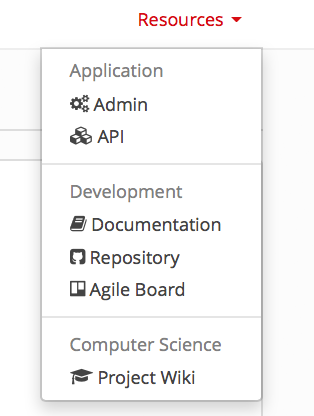
\includegraphics[scale=0.8]{figures/resource.png}
\caption{Drag-down menu for resources.}
\label{fig:resource}
\end{figure}
Besides the four dashboards we introduced above. Our visual design also provides a lot of resources related to our project in the resource menu on the top left. As shown in Figure~\ref{fig:resource}, we provide $6$ related resources: ``Admin'', ``API'', ``Documentation'', ``Repository'', ``Agile Board'' and ``Project wiki''.

\begin{figure*}
\centering
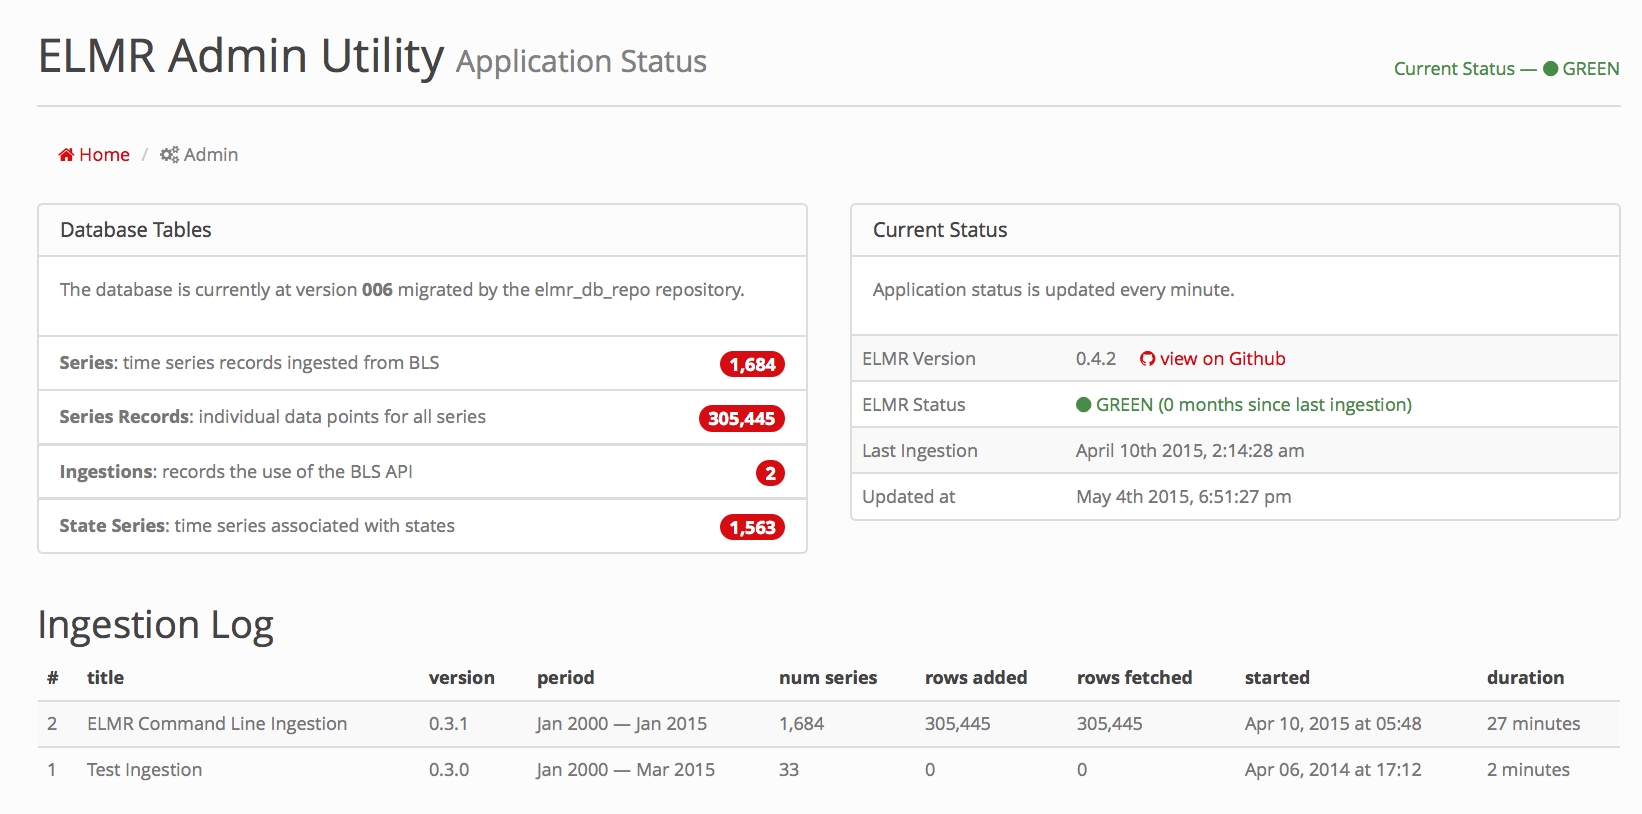
\includegraphics[scale = 0.5]{figures/Admin.png}
\caption{Illustration of Admin resources.}
\label{fig:admin}
\end{figure*}
As Figure~\ref{fig:admin} shows, in ``Admin'', the user can find the database information and current status of our project. It contains three parts. ``Database table'' shows the number of databases we downloaded. For example,  in Figure~\ref{fig:admin}, we see that we downloaded $1684$ time series data bases from website of BLS\cite{Labor_data}. Users can find the status of our ELMR project and the status of the database in ``Current status''. For example, user can find the version of our ELMR project is 0.4.2 and the latest update time of the project. ``Ingestion Log'' shows the (todo )

``API'' provides the url of the database we

``Documentation'' provides many useful information of developing our project. For example, in ``Ingestion'' part, it introduces the API of the website of BLS and list the series IDs of the most useful database. It also shows some sample code of how we make use of the API to fetch the data and show the data in a beautiful table. We believe that this kind of information is not only helpful for our team members to cooperate with each other, but also useful for other developers. User can also find the detailed instructions of how to run our project locally and some other interesting and useful information here.

Besides the above mentioned information. User cannot find the code of our project in ``Repository'', the progress report in ``Agile Board'' and our wiki page through ``Project Wiki''.

%This project will be primarily written in JavaScript using D3 \cite{D3} - it will be hosted on a website (with a small Python web server sending JSON data to the D3 front-end). It will also have a data ingestion component, allowing us to quickly gather data from the BLS and from the job release. It is our hope that our project will eventually be hosted by the Urban Institute and used widely by journalists and researchers.

\section{Usability Study}

To evaluate the usability of our ELMR for analyzing the employment situation, we recruited 8 participants to carry our usability study. All these participants are male PhD students from ECE or computer science department of UMD who has no professional knowledge of economics and labor force. Our usability study contains five main parts: background introduction, training, testing by completing research-driven tasks, testing by exploring features of user interests and questionnaire. The test takes around 10~15 minutes.

\subsection{Background Introduction}
We first give a very brief introduction of our project by showing a pre-recorded video. Since none of our participants is familiar with the employment data, we also introduce the three data sets we use: CPS, CES and LAU in a little more detail.


\subsection{Training}
To train the participants how to use ELMR, we first introduce the main components of the dashboard. Then we give an example of how to draw ``Employment ratio'' and ``employment-Population ratio'' using our time series data. During the training process, we encourage the participants to think-out-loud and ask any questions they cannot understand.

\subsection{Testing by Completing Research-Driven Tasks}
After the training session, the participants are asked to work on themselves to complete 5 research driven tasks using our tool. The eight questions are as follows:
\begin{enumerate}
\item    Show the time series of unemployment rate for Asian and White people. From 2008-2010, which group of people has higher relative changes of unemployment rate.

\item    which state has the highest unemployment rate in Oct. 2011
\item    In Mar 2011, which five states has the highest size of labor force, do they also have the highest employment level
\item     Show the time series of unemployment rate for Maryland and Florida
\item     Download a data set you are interested in.
\end{enumerate}

During the test session, we will record the time the participants spend on each of these questions. We encourage the user to think through each of these questions, telling us their thoughts when they try to answer each questions.

\subsection{Exploring User Interests feature}
After answering the 5 research driven questions. The participants are asked to propose one or two questions which are interests to them about the employment status of US and explore the answer their questions using our tool. Similarly, the participants are encouraged to think-out-loud, telling us any thoughts they have during answering the questions.

\subsection{questionnaire}
After finishing answering the above questions, the participants are asked to do a questionnaire which asks the participants to give their evaluation about our tool, and how difficult it is to answer each of our research driven questions.


\subsection{Results of Usability Test}
The typical responses of subjects regarding the questions are shown in the following:


\begin{enumerate}
\item    Show the time series of unemployment rate for As and white people. From 2008-2010, which group of people has higher relative changes of unemployment rate.


All of the subjects were able to answer this question by using the time series visualization, but they complained that if the y axis are aligned or they could put different series in one chart, they could have answered this kind of questions more efficiently.

\item    which state has the highest unemployment rate in Oct. 2011


When design this question, we suppose subjects to use the geography view to find the answer. However, since the wealth of nations part also visualize the unemployment rate of states over time, one subjects used this view to find the right answer. The other 4 subjects chose the geography view. Some of them complained that when the data of two states are very similar, they could not tell which one is bigger, so they suggested that when mouse is hovering on a state, the corresponding data should be shown for easier comparison. Most of the subjects were not happy with the the way they can choose the date, they wanted a time picker to pick a specific time point, but they all liked the slide bar because it enables them to see the animated change over time. In general, they all like the heat map since it is very visually informative and appealing.


\item    In Mar 2011, which five states has the highest size of labor force, do they also have the highest employment level?

This question is the most difficult question according to the feedback of users. They all attempted to answer this question using the Wealth of Nations view, but they still could not answer it quickly due to two reasons: it is pretty hard to choose time in this view, users have to be very careful about moving their mouse; the second reason is they are not sure what the size of the bubble stands for, so some of they were not able to answer the second part of the question.


\item     Show the time series of unemployment rate for Maryland and Florida
This seems to be an easy problem for the subjects, though two of them had a little difficulty to find these two data in the drop menu in the Time Series part, they were overwhelmed by the large dataset. They thought it would be good to organize the data or choose the data in a better fashion,

\item     Download a data set you are interested in.

Subjects finished this task very quickly, and they liked this feature because in this way, they can download the data they want and use other powerful visualization tools to find more insights.

\end{enumerate}

Based on the results of the usability study, we have improved our visualization with more functions like hints and more details to help users use it. For example, in the final version of our visualization, we have added a slide bar in the wealth of nations part to help users accurately select time. To help users compare two time series, we have aligned the x-axis of the . We also added an option to select different color scale in the heat map.

%\subsection{Usability Study Settings}
%Our usability test follow the guidelines stated in class:
%\begin{itemize}

%\item We conduct the test with several users using the "thinking aloud" method of data collection
%\item We ask several research driven questions and require users to find the answers with our tool
%\item The result of our study will be bugs, features, problems, etc. to add to our tool along with their severity and priority
%\end{itemize}


\section{Conclusion}
In this project, we design a web application to visualize the employment situation of the United States. This interface mainly contains 3 parts, a Time Series part to visualize and compare different statistics over time, a Geography part to visualize the employment situation for different states, an a wealth of nations part. It is developed mainly in JavaScript using D3, and a small Python web server is used to send JSON data to the D3 front-end. With a data ingestion component, it allows admins to gather data quickly from the BLS and from the monthly job release. Moreover, we conduct usability study to help improve the project development.

\section{Credit}

Benjamin Bengfort:

Xintong Han:

Assaf Magen:

Hao Zhou:


% Balancing columns in a ref list is a bit of a pain because you
% either use a hack like flushend or balance, or manually insert
% a column break.  http://www.tex.ac.uk/cgi-bin/texfaq2html?label=balance
% multicols doesn't work because we're already in two-column mode,
% and flushend isn't awesome, so I choose balance.  See this
% for more info: http://cs.brown.edu/system/software/latex/doc/balance.pdf
%
% Note that in a perfect world balance wants to be in the first
% column of the last page.
%
% If balance doesn't work for you, you can remove that and
% hard-code a column break into the bbl file right before you
% submit:
%
% http://stackoverflow.com/questions/2149854/how-to-manually-equalize-columns-
% in-an-ieee-paper-if-using-bibtex
%
% Or, just remove \balance and give up on balancing the last page.
%
\balance

% If you want to use smaller typesetting for the reference list,
% uncomment the following line:
% \small
\bibliographystyle{acm-sigchi}
\bibliography{paper}
\end{document}
